 
%%
%% This is file `sample-sigchi.tex',
%% generated with the docstrip utility.
%%
%% The original source files were:
%%
%% samples.dtx  (with options: `sigchi')
%% 
%% IMPORTANT NOTICE:
%% 
%% For the copyright see the source file.
%% 
%% Any modified versions of this file must be renamed
%% with new filenames distinct from sample-sigchi.tex.
%% 
%% For distribution of the original source see the terms
%% for copying and modification in the file samples.dtx.
%% 
%% This generated file may be distributed as long as the
%% original source files, as listed above, are part of the
%% same distribution. (The sources need not necessarily be
%% in the same archive or directory.)
%%
%% The first command in your LaTeX source must be the \documentclass command.
\documentclass[sigchi]{acmart}

\usepackage{spverbatim}
\usepackage{graphicx}
\usepackage{longtable}

%%
%% \BibTeX command to typeset BibTeX logo in the docs
%\AtBeginDocument{%%
%	\providecommand\BibTeX{{
%			\normalfont B\kern-0.5em{\scshape i\kern-0.25em b}\kern-0.8em\TeX}}}

%% Rights management information.  This information is sent to you
%% when you complete the rights form.  These commands have SAMPLE
%% values in them; it is your responsibility as an author to replace
%% the commands and values with those provided to you when you
%% complete the rights form.
\setcopyright{acmcopyright}
\copyrightyear{2018}
\acmYear{2018}
\acmDOI{10.1145/1122445.1122456}

%%
%% The majority of ACM publications use numbered citations and
%% references.  The command \citestyle{authoryear} switches to the
%% "author year" style.
%%
%% If you are preparing content for an event
%% sponsored by ACM SIGGRAPH, you must use the "author year" style of
%% citations and references.
%% Uncommenting
%% the next command will enable that style.
%%\citestyle{acmauthoryear}

%%
%% end of the preamble, start of the body of the document source.
\begin{document}
	
	%%
	%% The "title" command has an optional parameter,
	%% allowing the author to define a "short title" to be used in page headers.
	\title{Natural Language Processing CZ4045}
	\subtitle{Group Report (G20C)}
	
	%%
	%% The "author" command and its associated commands are used to define
	%% the authors and their affiliations.
	%% Of note is the shared affiliation of the first two authors, and the
	%% "authornote" and "authornotemark" commands
	%% used to denote shared contribution to the research.
	\author{Philipp Koch}
	\affiliation{%
		\institution{NTU - School of Computer Science and Engineering}
		\streetaddress{21 Lien Ying Chow Drive}
		\city{637296 Singapore}
		\country{Singapore}
	}
	\email{N1903454H@e.ntu.edu.sg}
	
	\author{Gantari Evanda Raufani}
	\affiliation{%
		\institution{NTU - School of Computer Science and Engineering}
		\streetaddress{30 Nanyang Crescent}
		\city{Singapore}
		\country{Singapore}
	}
	\email{gant0010@e.ntu.edu.sg}
	
	\author{Stella Marcella}
	\affiliation{%
		\institution{NTU - School of Computer Science and Engineering}
		\streetaddress{}
		\city{Singapore}
		\country{Singapore}
	}
	\email{smarcell001@e.ntu.edu.sg}
	
	\author{Dodda Sharon Olivia}
	\affiliation{%
		\institution{NTU - School of Computer Science and Engineering}
		\streetaddress{}
		\city{Singapore}
		\country{Singapore}
	}
	\email{sharonol001@e.ntu.edu.sg}
	
	\author{Janaki H Nair}
	\affiliation{%
		\institution{NTU - School of Computer Science and Engineering}
		\streetaddress{}
		\city{Singapore}
		\country{Singapore}
	}
	\email{janakih001@e.ntu.edu.sg}
	
	%%
	%% By default, the full list of authors will be used in the page
	%% headers. Often, this list is too long, and will overlap
	%% other information printed in the page headers. This command allows
	%% the author to define a more concise list
	%% of authors' names for this purpose.
	% \renewcommand{\shortauthors}{Trovato and Tobin, et al.}
	
	%%
	%% The abstract is a short summary of the work to be presented in the
	%% article.
	\begin{abstract}
		Our task covered data processing on a dataset provided by the review platform \textit{yelp}. We had to analyze the data
		descriptively and we had to focus on the Adjectives in the reports. Therefore we had to compare different methods on how the reviews can be represented by adjectives, which also became our application model. In our application model we were able to find specific properties of the business reviewed in the data.
	\end{abstract}
	
	%%
	%% The code below is generated by the tool at http://dl.acm.org/ccs.cfm.
	%% Please copy and paste the code instead of the example below.
	%%
	\begin{CCSXML}
		<ccs2012>
		<concept>
		<concept_id>10010520.10010553.10010562</concept_id>
		<concept_desc>Computer systems organization~Embedded systems</concept_desc>
		<concept_significance>500</concept_significance>
		</concept>
		</ccs2012>
	\end{CCSXML}
	
	\ccsdesc[500]{Natural Language Processing~Group Assignment}

	
	%%
	%% Keywords. The author(s) should pick words that accurately describe
	%% the work being presented. Separate the keywords with commas.
	\keywords{datasets, neural networks, gaze detection, text tagging}
	
	
	%%
	%% This command processes the author and affiliation and title
	%% information and builds the first part of the formatted document.
	\maketitle
	
	\section{Dataset Analysis}
	\subsection{Writing Style}
	For our analysis of the writing style, we picked some random sentences as a sample to compare it with articles in the well known newspaper “The Strait Times”, whereby we used the food section as a control sample. The list below shows our observations:
\linebreak

\begin{itemize}
    \item The last sentence does not have a final punctuation.
    \item The review lacks proper punctuation in the sentences.
    \item There is usage of words that are not in the English dictionary.
    \item There is use of slang. 
    \item The first words of the sentences in the review are not capitalized.
    \item The last sentence does not have a final punctuation.
    \item News articles are usually written in third person point of view, however the reviews from yelp are written in first person point of view.
    \item The first words of the sentences in the review are not capitalized.
    \item The last sentence does not have a final punctuation.
    \item News articles are usually written in third person point of view, however the reviews from yelp are written in first person point of view.
    \item The review contains onomatopoeia.
    \item The review uses all capitalised characters to create emphasis.
    \item News articles usually do not contain punctuation like ‘...’ that suggests pause.
    \item Words like ‘gal’ that is used to denote a girl is considered informal which is used in the review but not a news article.
    \item News articles usually use subject-verb-object construction for the sentences.
    \item The review contains many exclamation marks for one sentence although it is not necessary (known as “exclamation-point inflation” in digital communication).
    \item Some of the first words in sentences like ‘the’ are not capitalized.
    \item Personal pronouns like ‘i’ aren't capitalized.
    \item There are misspelled words, such as ‘espically’.
    \item There are missing punctuation in the reviews.
    \item The review is not relevant to the business.
    \item The review is not in full proper sentences.
    \item The review contains smileys (~2 \% of all reviews contain smileys).
\end{itemize}

	\subsection{Sentence Segmentation}
	For the sentence segmentation we used the library spacy. Each category is displayed in figure 1.
	\begin{center}
		\begin{table}[!h]
			\caption{Average length of the sentences in the different star categories}
			\begin{tabular}{ c c c c c}
				1 Star & 2 Star & 3 Star  & 4 Star & 5 Star\\
				30.5 & 25.9 & 24.0  & 25 & 24\\
			\end{tabular}
		\end{table}
	\end{center}
	
	\begin{figure}
		\caption{Histograms of the length of the sentences}
		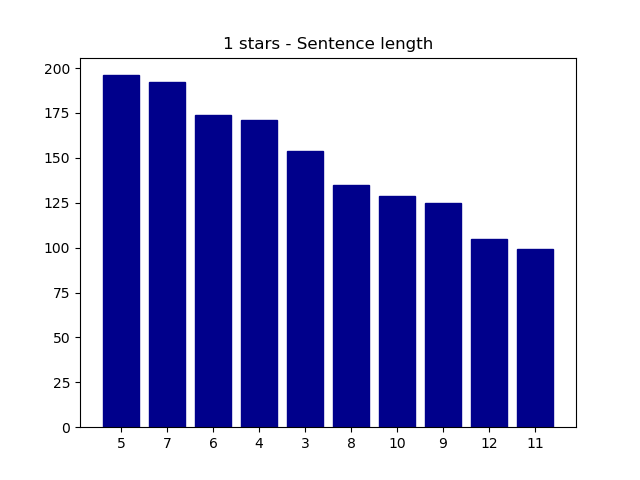
\includegraphics[scale=0.3]{figures/1stars-Sentencelength.png}
		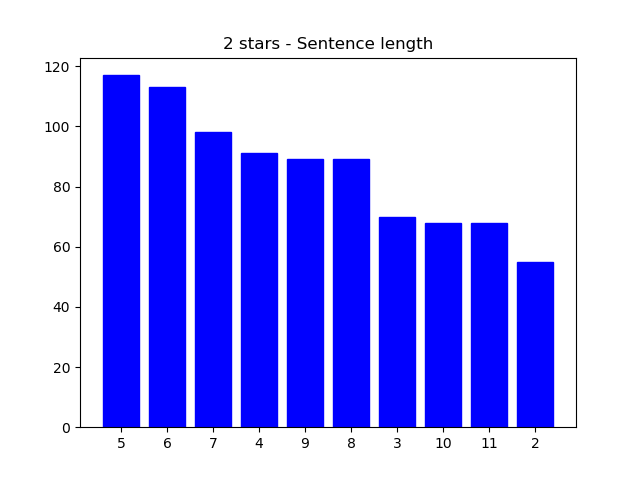
\includegraphics[scale=0.3]{figures/2stars-Sentencelength.png}
		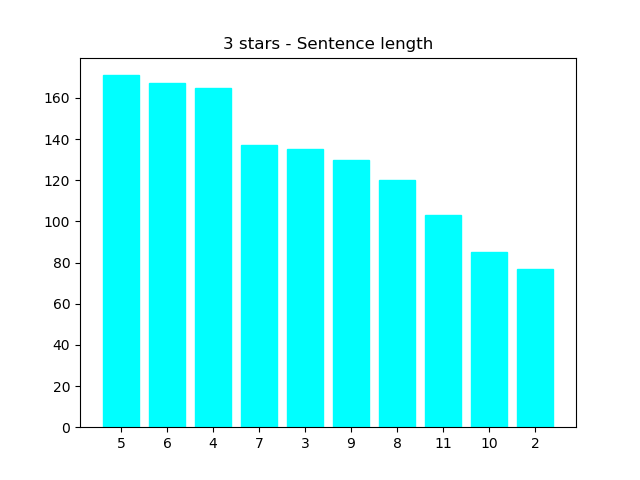
\includegraphics[scale=0.3]{figures/3stars-Sentencelength.png}
		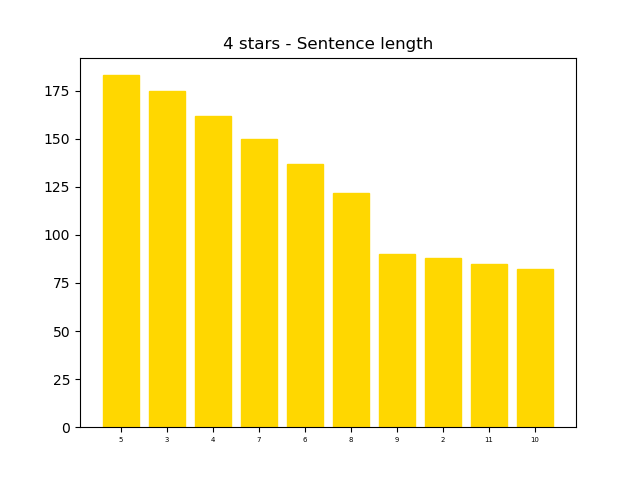
\includegraphics[scale=0.3]{figures/4stars-Sentencelength.png}
		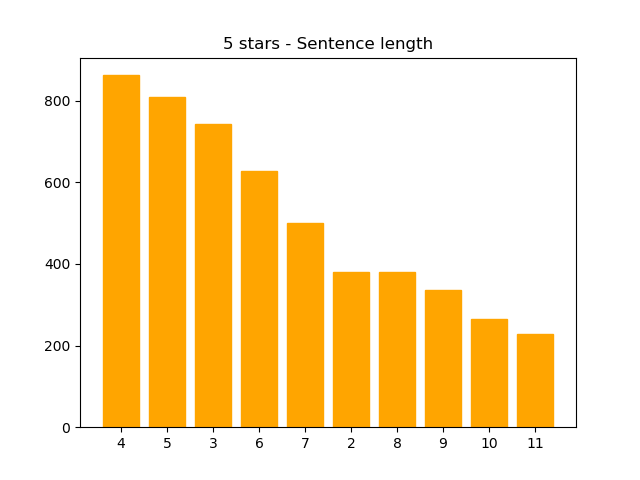
\includegraphics[scale=0.3]{figures/5stars-Sentencelength.png}
	\end{figure}
	As can be seen, the length of sentences is on average longer with a poor rating than with a good rating. 
	
	\subsection{Tokenization and Stemming}
	For this task, we used the NLTK library to calculate the number of unique tokens that exist in a review. Then, we plotted the graphs to show the distributions of the tokens, both with and without stemming.

We can see the figure below. Figure 2 shows the number of unique tokens without stemming in every review, while Figure 3 shows the number of unique tokens after stemming is performed in every review. To make the comparison easier, in Figure 4, the stems are indicated with the color orange, while the tokens are indicated with the color blue.

Based on Figure 4, we can conclude that the number of unique tokens with stemming is generally lower that the number of unique tokens without performing stemming.

\begin{figure}
    \caption{Distributions of tokens in each review (without stemming)}
    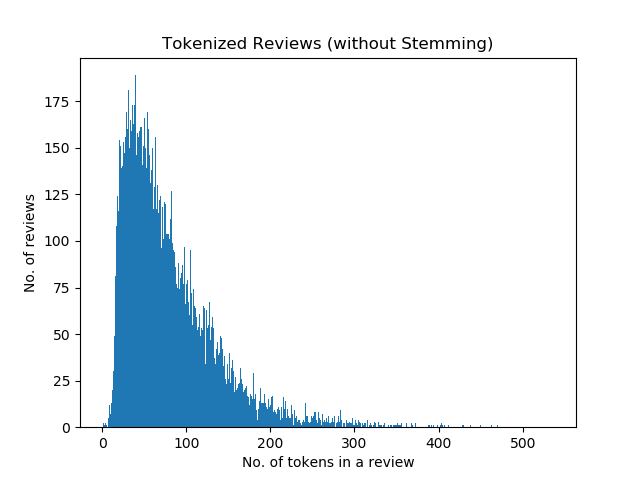
\includegraphics[scale=0.5]{token_review.png}
    \label{fig:tokenized_review}
\end{figure}

\begin{figure}
    \caption{Distributions of tokens in each review (with stemming)}
    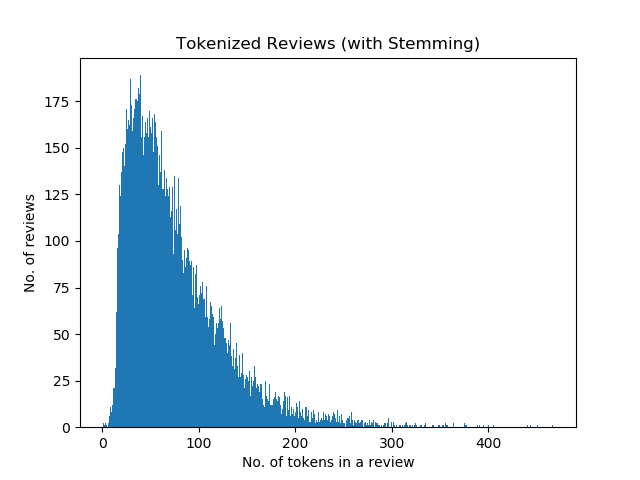
\includegraphics[scale=0.5]{stem_review.png}
    \label{fig:stemmed_token_review}
\end{figure}

\begin{figure}
    \caption{Comparison of the distributions of the tokens with and without stemming}
    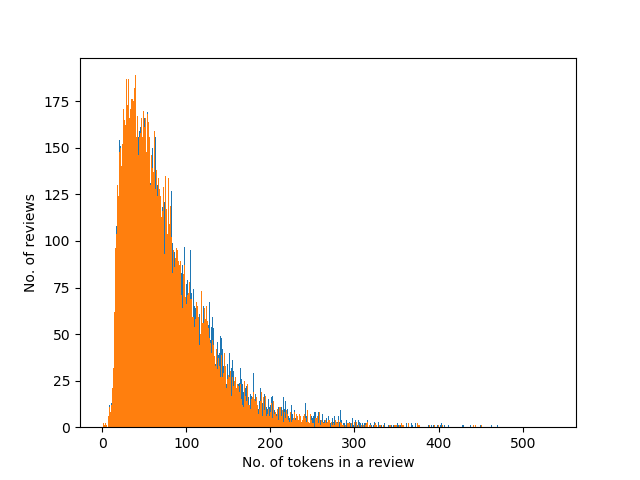
\includegraphics[scale=0.5]{token_stem_review.png}
    \label{fig:stem_and_token_review}
\end{figure}

\begin{table}[]
    \centering
    \begin{tabular}{c|c}
         &  \\
         & 
    \end{tabular}
    \caption{Caption}
    \label{tab:my_label}
\end{table}
	\clearpage
	\subsection{POS Tagging}
	For the POS tagging, we used the word\_tokenize() function from the nltk library. The table below shows the results of POS tagging 5 random reviews.

\setlength{\tabcolsep}{18pt}
\renewcommand{\arraystretch}{1.75}
    \begin{longtable}{| p{3cm} | p{3cm} |} 
    	
        \hline 
         \textbf{Review/Text} & \textbf{Parts of Speech} \\ [0.5ex] 
         \hline
         The bubble tea was excellent! The service however, was not. I found it pushy, rushed, abrasive, and incredibly rude. Their way of dealing with English speaking customers is to bark at them until they leave with their order. You certainly won't be receiving any of my money ever again. & [('The', 'DT'), ('bubble', 'JJ'), ('tea', 'NN'), ('was', 'VBD'), ('excellent', 'JJ'), ('!', '.'), ('The', 'DT'), ('service', 'NN'), ('however', 'RB'), (',', ','), ('was', 'VBD'), ('not', 'RB'), ('.', '.'), ('I', 'PRP'), ('found', 'VBD'), ('it', 'PRP'), ('pushy', 'VBZ'), (',', ','), ('rushed', 'VBD'), (',', ','), ('abrasive', 'JJ'), (',', ','), ('and', 'CC'), ('incredibly', 'RB'), ('rude', 'VB'), ('.', '.'), ('Their', 'PRP\$'), ('way', 'NN'), ('of', 'IN'), ('dealing', 'VBG'), ('with', 'IN'), ('English', 'NNP'), ('speaking', 'VBG'), ('customers', 'NNS'), ('is', 'VBZ'), ('to', 'TO'), ('bark', 'VB'), ('at', 'IN'), ('them', 'PRP'), ('until', 'IN'), ('they', 'PRP'), ('leave', 'VBP'), ('with', 'IN'), ('their', 'PRP\$'), ('order', 'NN'), ('.', '.'), ('You', 'PRP'), ('certainly', 'RB'), ('wo', 'MD'), ("n't", 'RB'), ('be', 'VB'), ('receiving', 'VBG'), ('any', 'DT'), ('of', 'IN'), ('my', 'PRP\$'), ('money', 'NN'), ('ever', 'RB'), ('again', 'RB'), ('.', '.')] \\ 
         \hline
         I love the sketch comedy nights! Food is not so great. Drinks are average prices. Good venue. & [('I', 'PRP'), ('love', 'VBP'), ('the', 'DT'), ('sketch', 'NN'), ('comedy', 'NN'), ('nights', 'NNS'), ('!', '.'), ('Food', 'NNP'), ('is', 'VBZ'), ('not', 'RB'), ('so', 'RB'), ('great', 'JJ'), ('.', '.'), ('Drinks', 'NNS'), ('are', 'VBP'), ('average', 'JJ'), ('prices', 'NNS'), ('.', '.'), ('Good', 'JJ'), ('venue', 'NN'), ('.', '.')] \\
         \hline
         This place is inside Baiz Supermarket. If you are in mood of middle eastern food, this is the place. They have the most popular dishes. I highly recommend this place! & [('This', 'DT'), ('place', 'NN'), ('is', 'VBZ'), ('inside', 'JJ'), ('Baiz', 'NNP'), ('Supermarket', 'NNP'), ('.', '.'), ('If', 'IN'), ('you', 'PRP'), ('are', 'VBP'), ('in', 'IN'), ('mood', 'NN'), ('of', 'IN'), ('middle', 'JJ'), ('eastern', 'JJ'), ('food', 'NN'), (',', ','), ('this', 'DT'), ('is', 'VBZ'), ('the', 'DT'), ('place', 'NN'), ('.', '.'), ('They', 'PRP'), ('have', 'VBP'), ('the', 'DT'), ('most', 'RBS'), ('popular', 'JJ'), ('dishes', 'NNS'), ('.', '.'), ('I', 'PRP'), ('highly', 'RB'), ('recommend', 'VBP'), ('this', 'DT'), ('place', 'NN'), ('!', '.')] \\
         \hline
         I used to love Jukebox but after today's meal, all I can say is "it was nice while it lasted". That was the dryest, most flavorless burger I've ever had. The cook didn't even bother getting the patty all on the bun, but just slapped everything together in a sloppy, careless mess. The fries were way overcooked (it used to come with curly but those are now an extra \$\$). The bun was plain, untoasted and there was no tomato (there was supposed to be). \$18 for overpriced cardboard. & [('I', 'PRP'), ('used', 'VBD'), ('to', 'TO'), ('love', 'VB'), ('Jukebox', 'NNP'), ('but', 'CC'), ('after', 'IN'), ('today', 'NN'), ("'s", 'POS'), ('meal', 'NN'), (',', ','), ('all', 'DT'), ('I', 'PRP'), ('can', 'MD'), ('say', 'VB'), ('is', 'VBZ'), ('``', '``'), ('it', 'PRP'), ('was', 'VBD'), ('nice', 'RB'), ('while', 'IN'), ('it', 'PRP'), ('lasted', 'VBD'), ("''", "''"), ('.', '.'), ('That', 'DT'), ('was', 'VBD'), ('the', 'DT'), ('dryest', 'JJS'), (',', ','), ('most', 'JJS'), ('flavorless', 'JJ'), ('burger', 'NN'), ('I', 'PRP'), ("'ve", 'VBP'), ('ever', 'RB'), ('had', 'VBN'), ('.', '.'), ('The', 'DT'), ('cook', 'NN'), ('did', 'VBD'), ("n't", 'RB'), ('even', 'RB'), ('bother', 'VB'), ('getting', 'VBG'), ('the', 'DT'), ('patty', 'NN'), ('all', 'DT'), ('on', 'IN'), ('the', 'DT'), ('bun', 'NN'), (',', ','), ('but', 'CC'), ('just', 'RB'), ('slapped', 'VBD'), ('everything', 'NN'), ('together', 'RB'), ('in', 'IN'), ('a', 'DT'), ('sloppy', 'JJ'), (',', ','), ('careless', 'JJ'), ('mess', 'NN'), ('.', '.'), ('The', 'DT'), ('fries', 'NNS'), ('were', 'VBD'), ('way', 'NN'), ('overcooked', 'VBN'), ('(', '('), ('it', 'PRP'), ('used', 'VBD'), ('to', 'TO'), ('come', 'VB'), ('with', 'IN'), ('curly', 'JJ'), ('but', 'CC'), ('those', 'DT'), ('are', 'VBP'), ('now', 'RB'), ('an', 'DT'), ('extra', 'JJ'), ('\$', '\$'), ('\$', '\$'), (')', ')'), ('.', '.'), ('The', 'DT'), ('bun', 'NN'), ('was', 'VBD'), ('plain', 'RB'), (',', ','), ('untoasted', 'JJ'), ('and', 'CC'), ('there', 'EX'), ('was', 'VBD'), ('no', 'DT'), ('tomato', 'NN'), ('(', '('), ('there', 'EX'), ('was', 'VBD'), ('supposed', 'VBN'), ('to', 'TO'), ('be', 'VB'), (')', ')'), ('.', '.'), ('\$', '\$'), ('18', 'CD'), ('for', 'IN'), ('overpriced', 'VBN'), ('cardboard', 'NN'), ('.', '.')] \\
         \hline
         Scheduled manicure and pedicure one day. Came in, was seated and was told to wait. Waited for over 30 minutes, went back to the front desk, they said they forgot about me. I was nice about it, I guess that happenes (not at the good places, but still happens). At the end wasn't even offered a discount... pretty shitty move. & [('Scheduled', 'VBN'), ('manicure', 'NN'), ('and', 'CC'), ('pedicure', 'NN'), ('one', 'CD'), ('day', 'NN'), ('.', '.'), ('Came', 'NN'), ('in', 'IN'), (',', ','), ('was', 'VBD'), ('seated', 'VBN'), ('and', 'CC'), ('was', 'VBD'), ('told', 'VBN'), ('to', 'TO'), ('wait', 'VB'), ('.', '.'), ('Waited', 'VBN'), ('for', 'IN'), ('over', 'IN'), ('30', 'CD'), ('minutes', 'NNS'), (',', ','), ('went', 'VBD'), ('back', 'RB'), ('to', 'TO'), ('the', 'DT'), ('front', 'NN'), ('desk', 'NN'), (',', ','), ('they', 'PRP'), ('said', 'VBD'), ('they', 'PRP'), ('forgot', 'VBD'), ('about', 'IN'), ('me', 'PRP'), ('.', '.'), ('I', 'PRP'), ('was', 'VBD'), ('nice', 'JJ'), ('about', 'IN'), ('it', 'PRP'), (',', ','), ('I', 'PRP'), ('guess', 'VBP'), ('that', 'IN'), ('happenes', 'NNS'), ('(', '('), ('not', 'RB'), ('at', 'IN'), ('the', 'DT'), ('good', 'JJ'), ('places', 'NNS'), (',', ','), ('but', 'CC'), ('still', 'RB'), ('happens', 'VBZ'), (')', ')'), ('.', '.'), ('At', 'IN'), ('the', 'DT'), ('end', 'NN'), ('was', 'VBD'), ("n't", 'RB'), ('even', 'RB'), ('offered', 'VBN'), ('a', 'DT'), ('discount', 'NN'), ('...', ':'), ('pretty', 'RB'), ('shitty', 'JJ'), ('move', 'NN'), ('.', '.')] \\  
         \hline
    \end{longtable}

    


	\subsection{Most Frequent Adjectives for each Rating}
	\section{Development of a <Noun - Adjective> Pair Summarizer}
	The results are displayed in Table 6 and Table 7.
\subsection{Approach}
For the extraction of the Noun-Adjectives, we used a dependency-grammar approach. In dependency grammar, relations with adjectives are labeled as 'amod' for sentences like "... bad service ..." while in the case of Adjectives in sentences like "... the service at ... is bad ...", the adjectives are labeled as 'acomp'. With this two labels we were able to identify the adjectives. In the case of 'amods', the parent node is checked for being a Noun. If there is a POS-tagged 'NOUN' here, the pair is found. For 'acomp' adjectives all child nodes of the parent node were checked. If there is a relation 'nsubj' here, the pair is found. Before adding the pairs, the words are being lemmatized so the result is a more accurate number of the used words. We decided to do so since our corpus is to small to distinct between different tenses. To prevent incorrect POS tagged words from being included in the results, lemmatization takes place after identification. All of these relations were being stored in an array.\\
\begin{Verbatim}[fontsize=\tiny]
# the case that the adjective is a direct amod
if token.dep_ == 'amod' and token.pos_ == "ADJ":
	if token.head.pos_ == 'NOUN':

		# lemmatize the tokens
		if token.head.lemma_ == '-PRON-':
			pair = ( token.lemma_.lower(), e.text.lower() )
		else:
			pair = ( 
				token.lemma_.lower(), 
				token.head.lemma_.lower() 
				)
		pairs.append(pair)

# the case that the adjective is a adj complement
if token.dep_ == 'acomp' and token.pos_ == "ADJ":
	noun = [
		e for e in token.head.children if e.dep_ == "nsubj"
		]
	if noun:
		for e in noun:

		# skip non nouns
		if not e.pos_ == 'NOUN':
		continue

		# lemmatize the tokens
		if e.lemma_ == '-PRON-':
			pair = ( token.lemma_.lower(), e.text.lower() )
		else:
			pair = ( token.lemma_.lower(), e.lemma_.lower() )
			pairs.append(pair)
\end{Verbatim}
\subsection{Analysis}
The pairs created for Business 1 are indicating already the sector of the company. Pairs like ('clean', 'car'), ('basic', 'wash') or ('classic', 'wash') are signs, that we are dealing with the reviews of a car wash here. After reviewing the texts, it became clearer that opinions about this business are mixed. Costumers mentioned bad service, which is also indicated by the determined pairs, like ('poor', 'job'), ('terrible', 'job') or ('bad', 'service'). In contrast, there were also some good reviews about this business, which also came up in the pairs. The most common pair is, for example, ('clean', 'car'), which indicates a good service. In total the results are satisfying, since most of the pairs are providing useful information. The only exception here is ('high', 'pressure') which is too ambiguous.\\
Business 2 was also a non restaurant business. The noun-adjective pairs such as ('front’,’desk’), ('free’,’wifi’), ('rental’, 'car’), ('complimentary’, 'breakfast’) suggest that the reviews are about an hotel which is true. We also get a general idea from the pairs that the staff, breakfast as well as the facilities are decent which is also true from reading the reviews. Apart from some complaints here and there in the reviews, the guests generally liked the hotel and its free shuttle service. However, some pairs like ('light’, 'sleeper’) is useless as it talks about the guest. Also, ('next’, 'day’) and ('first’, 'day’) occur frequently which does not give us any info.\\
As for Business 3, most reviews spoke great of the dumplings as well as the food, which are the 2 most frequent noun-adjective pairs. Hence, those are accurate. As from the reviews, it is given that the restaurant has a mix of Korean as well as Northern-Chinese dishes which is also something that can be rightly perceived from the frequent noun-adjective pairs obtained, e.g, ('korean’, 'food’), ('korean’, 'dishes’), ('chinese’, 'cuisine’), etc. Fried pork and fried rice are some of the dishes that are sold in the restaurant that people talked of in the reviews. Most reviews talk of how bad the service is. Apparently, the management and staff is not friendly, and the food is brought in quite slowly. This is in contradiction with one of the noun-adjective pairs that we got (('great’), ('service’)).  Perhaps, the noun-adjective pair could not comprehend the meaning of the sentences where service and great would appear together. These are some sentences quoted from the reviews: “If you are expecting great service, this the wrong place for you”, “but service is not so great”.  Therefore, when extracting noun-adjective pairs for these sentences, we obtain ('great’), ('service’), although the expression of the sentence is actually negative.\\
Business 4 represents a South Indian restaurant with a buffet set-up. Hence, the first three most frequent adj-noun pairs correctly summarizes the nature of the restaurant and the kind of food being served in the restaurant. Noun-adj pairs like ('first’, 'time’) do not hold much importance in the feedback of the restaurant but ('second’, 'time’) can refer to customers wanting to come back which speaks good of the restaurant. Besides, this is quite true because there are quite a few reviews that talks about customers wanting to give it another try. Most reviews also speak good of the staff as given by the ('friendly’, 'staff’) pair. Most spoken of food item is the dosa and that’s also given as one of the noun-adjective pairs. On the whole, the frequent noun-adjective pairs obtained give an accurate response of the restaurant.\\
For business 5, the determined pairs are providing useful information. A strong point here is that we don't have pairs related to time. The second most often pair is ('mexican', 'food') and the other pair is ('mexican', 'restaurant'), we can easy infer, that this business is a mexican restaurant. The inspection of the reviews proofed this assumption. Most of these reviews were positive towards the business. Determined pairs like ('great', 'place'), ('authentic','food') or ('best','food') emphasizing this observation.In the reiews many little things are mentioned, which is also reflected in the determined pairs. There are examples such as ('carne', 'asada'), ('toasted', 'bread') and ('iced', 'tea'), which indicate such peculiarities. The generated pairs for Business 5 are very unambiguous, so all pairs can be used to retrieve information.
	

	
\subsection{Conclusion}
With this summary we were able to find very specific characteristics of the businesses. There are many useful adjectives for the specific offers of the restaurant (e.g: ((('best', 'buffet'), 4), ((('quick', 'service'), 2), ('good', 'food'), 5))). With these results we can extract the most important pairs of reviews. But there are still some pairs that are not useful for extracting the main information of the reviews, such as time information that is not meaningful without its context( e.g.: (("single", "time"), 2),(("first", "night"), 3), ((("first", "day"), 2)) ). We assume that the reason for this is the problem of ambiguity in POS tagging. Neither NLTK nor Spacy were able to distinguish between the function of a determiner and an adjective. Since these time words can also be used as adjectives in other contexts, an exclusion of these words would not be reasonable. There were also some inaccuracies like (("tomato", "sauce"), 3), which are not useful for reflection.
In conclusion we can state, that we can extract many useful information with this Noun-Adjective Pair Summarizer.
	\section{Application}
	
\end{document}
\endinput
%%
%% End of file `sample-sigchi.tex'.
 
